\chapter{Hamiltonian flow}



\section{Basics}


In this section, we will define curves and vector field following the 
approach adopted in Secs.~2.5, 2.6 and 2.7 of Ref.~\cite{schutz1980geometrical}.



\subsection{Curve}

A curve $C$ is a mapping from $\mathbb{R}$ to a manifold $M$, $C: \mathbb{R} \rightarrow  M$.
This is illustrated in Fig.~\ref{curve}. Note that two curves need not be the same 
even if they map to the same image in $M$. For example, the curves $C_1$ and $C_2$
are not the same in Fig.~\ref{curve}. This is so because their
pre-images (elements of the domain $\mathbb{R}$
corresponding to an image in $M$) are different.




\begin{figure}
   \centering
  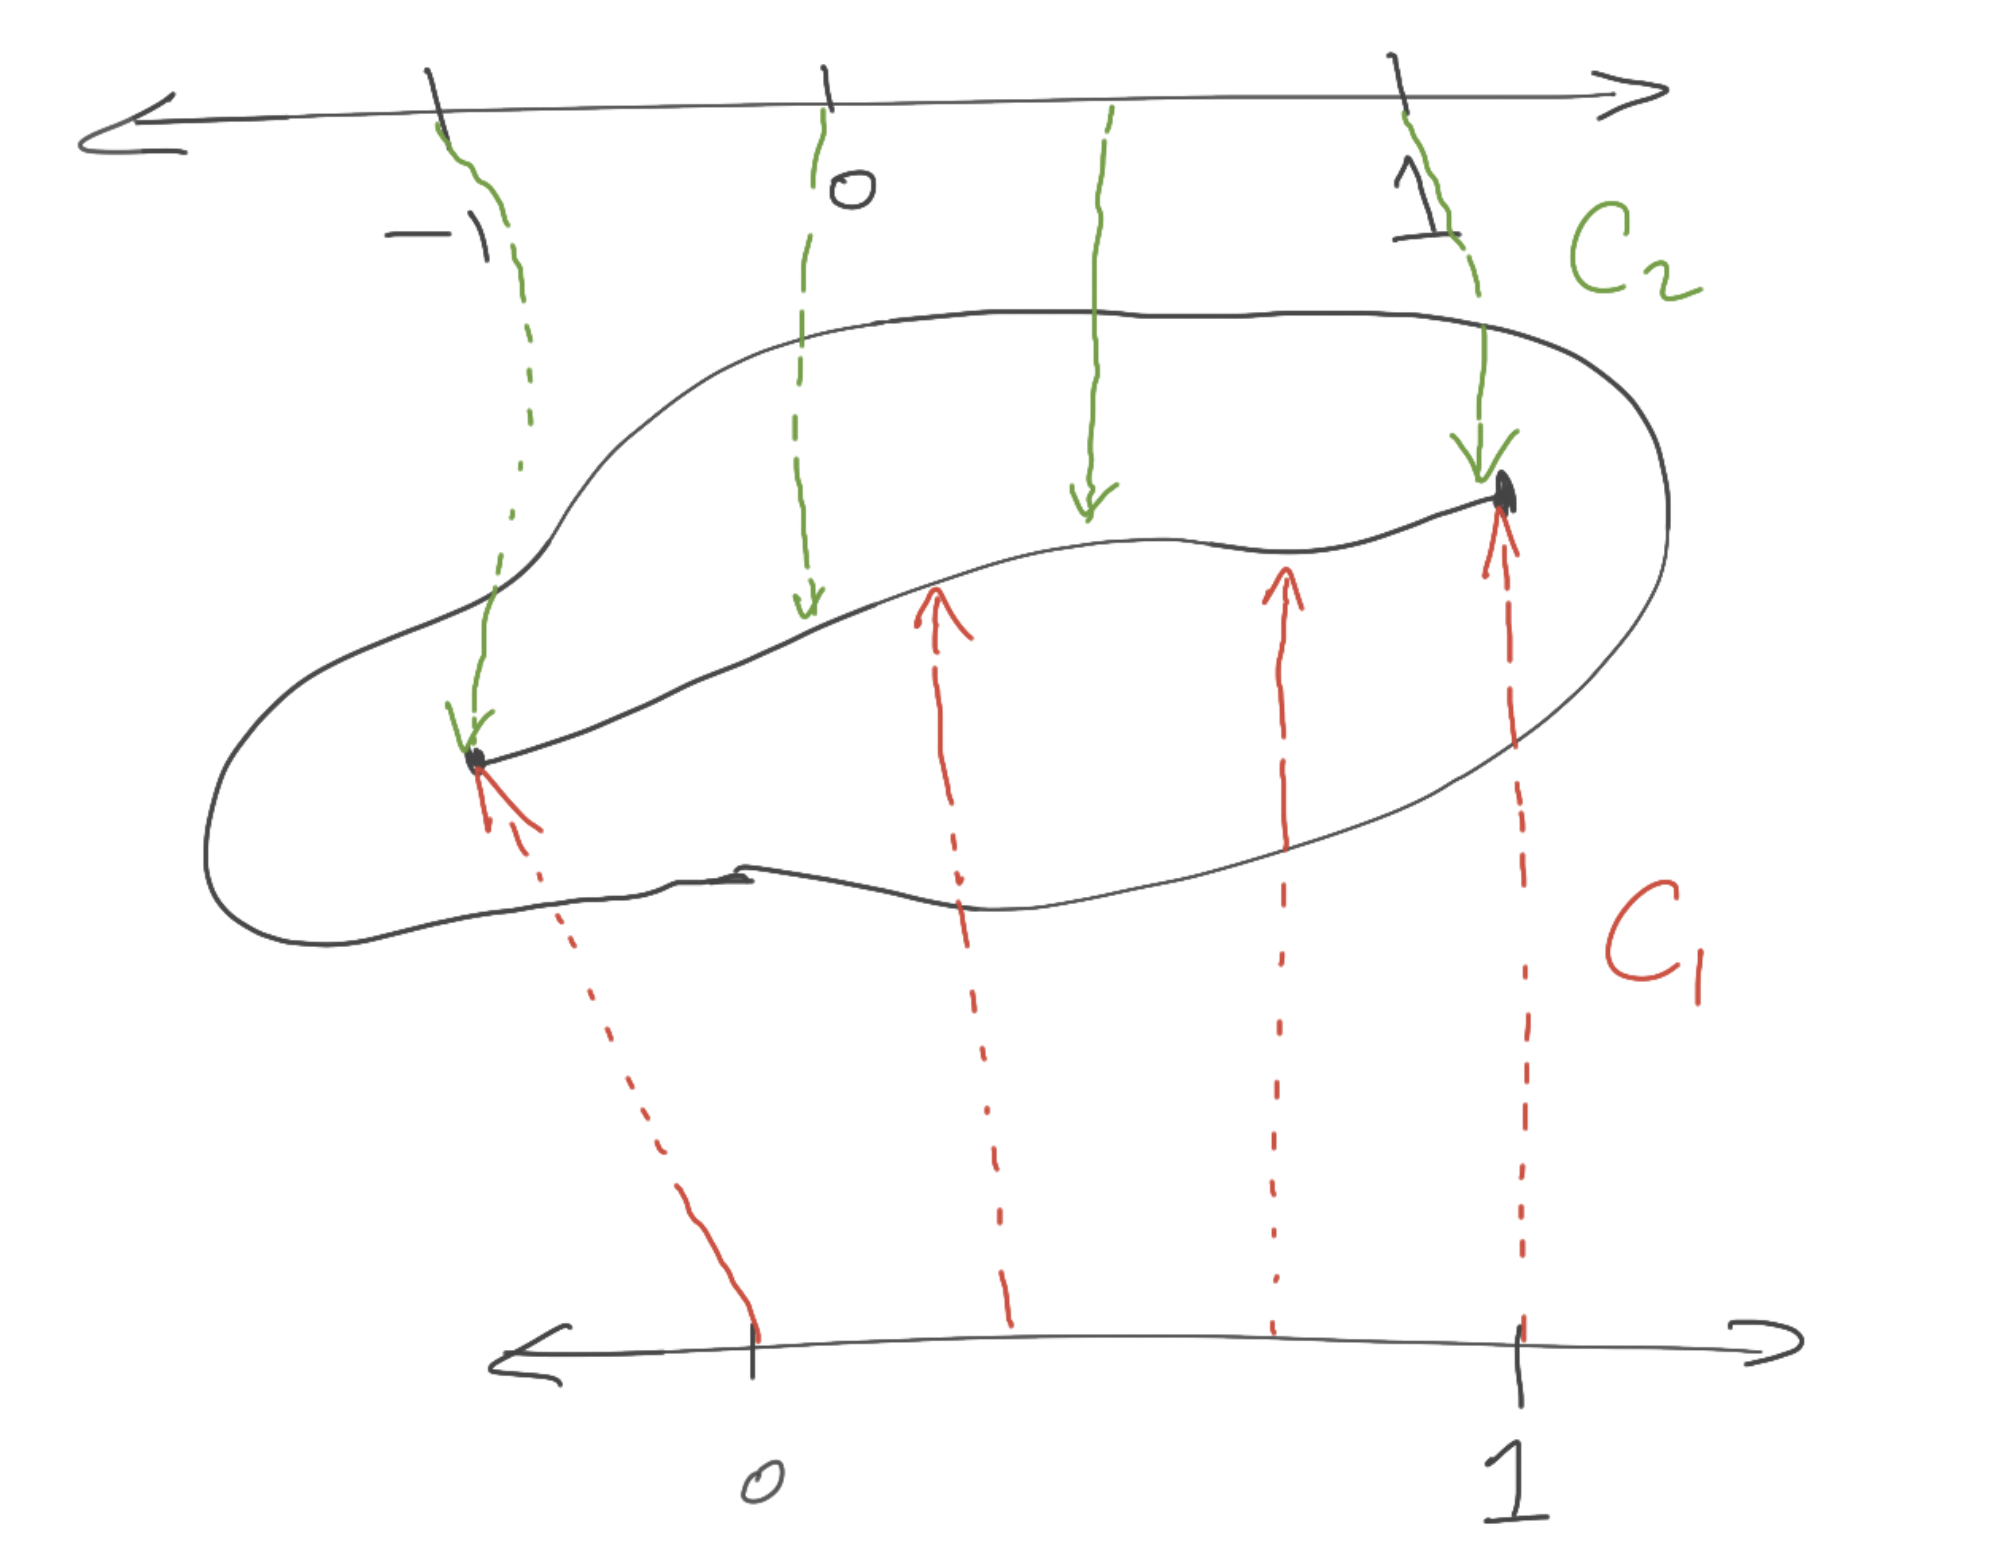
\includegraphics[width=0.4\linewidth]{curve}
  \caption{Pictorial  depiction of the concept of  a curve. 
  We are showing two different curves $C_1$ and $C_2$ which have the same image
  in manifold $M$.
    \vspace{-1.em}
  }
  \label{curve}
\end{figure}




\subsection{Vector field}


Imagine a curve $C$ defined by equations 
$\vv{x} = \vv{x}(\lambda)$ ($\vv{x}$ being the vector
of coordinates on $M$ and $\lambda  \in  \mathbb{R} $
 being the pre-image of $C$). Then at a point $P$ through which 
 the curve passes, we can 
define a vector whose components are $(dx^i/d \lambda)$. 
This vector (tangent to curve $C = x^i(\lambda)$)
is also denoted by $d/d \lambda$. After all,
 a vector is basically  a derivative operator.
This way we define vectors at every point of a curve $C$. If there are curves permeating
the manifold $M$, this can help us define a unique vector field on $M$, provided 
these curves don't intersect. A pictorial representation is shown in 
Fig.~\ref{vector_field}.




\begin{figure}
   \centering
  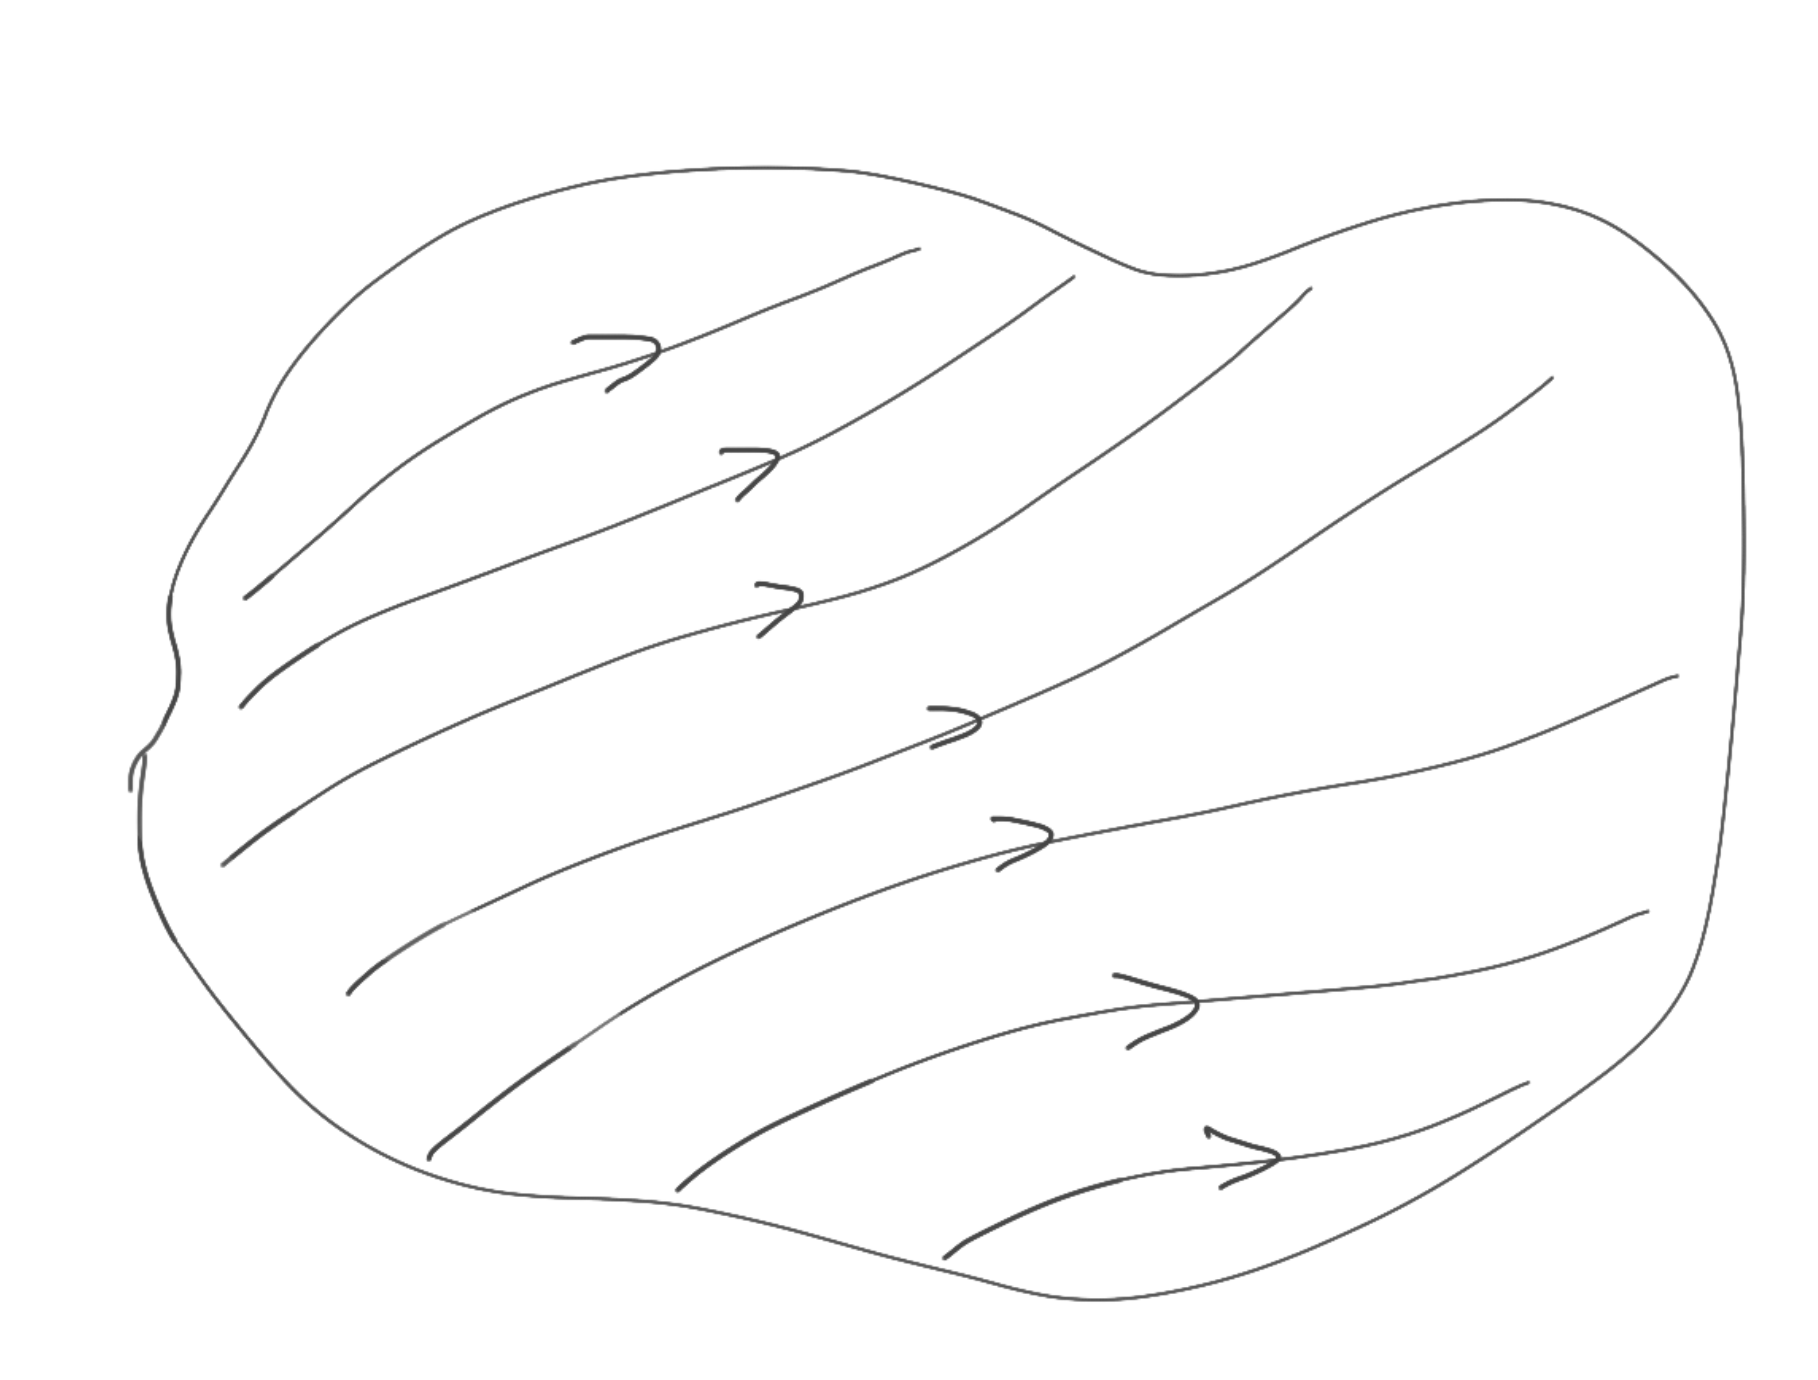
\includegraphics[width=0.4\linewidth]{vector_field}
  \caption{A manifold permeated with curves is a manifold with a vector field.
  These set of curves are also collectively refereed to as the flow of the
  associated vector field.
    \vspace{-1.em}
  }
  \label{vector_field}
\end{figure}


\section{Hamiltonian vector field and flow}

Unless stated otherwise, $\vv{V}$ from now on represents a column vector 
which contains all the components of $\vv{R}, \vv{P}, \vv{S}_1$ and $\vv{S}_2$.
Now, at all the points of the phase-space (which is a legitimate manifold),
we can define curves for a function $f(\vec{V})$ via (parameterized by $\lambda$)
\begin{align}
\frac{d \vv{V}}{d \lambda}   =  \pb{\vv{V},  f}  .       \label{H-flow}
\end{align}
It's implied that the above equation is to
 be interpreted in a component-wise manner.
The resulting vector field from these curves is called the 
\textit{Hamiltonian vector field} of $f$. Note that if $f = H$, then we will
have the Hamiltonian vector field of the 
Hamiltonian. More generally, with this definition, 
the Hamiltonian vector field of position 
$R_x$, momentum $P_z$ and the Hamiltonian $H$
are all well defined mathematical entities. 
For brevity we may refer to 
Hamiltonian flow as only the flow. 
Also note that under the flow of $f$, another quantity 
$g$ (both $f$ and $g$ being functions of the
phase space coordinates $V_i$) changes as
\begin{align}           \label{flow_eqn_2}
\frac{d g(V_k)}{d \lambda} =  \frac{\pd g}{\pd V_k} \frac{\pd V_k}{\pd \lambda}=           
\frac{\pd g}{\pd V_k}    \pb{V_k, f}   = \pb{g, f}    , 
\end{align}
where $V_k$ refers to all the phase space coordinates of the system
and use of the chain rule for PBs has been made in the second-last equality; see
Eq.~\eqref{C0-PBs_defined_2}.
Eq.~\eqref{flow_eqn_2}   
specializes to Eq.~\eqref{C0-EOM-PB} for a flow under the Hamiltonian.






The \textsc{Mathematica} notebook for evaluating the Poisson 
brackets between two general quantities 
is available at Ref.~\cite{MMA1} and 
\href{https://youtu.be/aoiCk5TtmvE}{this} YouTube video 
shows how to use this package.




\hfill \break


\begin{definition}[label=def:BB]
\textbf{Hamiltonian vector field:}
See Refs.~\cite{jose, arnold} for a more highbrow but
equivalent definition of Hamiltonian vector fields
using symplectic forms.
\end{definition}

\hfill \break




\begin{Exercise}    \label{exercise-2}
\textbf{Problem:}  Draw pictures representing the Hamiltonian
flows of $R_x, P_x, L_x, L^2,$ and $J^2$.



\textbf{Solution:} 

For this exercise let $\vv{V}$ represent the totality of 
coordinates contained in $\vv{R}, \vv{P}, \vv{S}_1$ and $\vv{S}_2$,
unless stated otherwise.
We will give the mathematical
 solution for only the first flow (in addition to the
pictorial representation of the flow).
Solutions for the other flows will not be given; they are quite
simple to obtain.
Also the associated figures representing the flows,
the arrows denote the direction of
increasing flow parameter, i.e. $\lambda$.






\textbf{(a)}

Under the flow of $R_x$, among all the
coordinates of $\vv{V}$, only $P_x$ changes via
\begin{align}
\frac{d P_x}{d \lambda}  =  \pb{P_x, R_x} = -1,
\end{align}
since the PB of $R_x$ with all other variables is 0. 
The solution is $ P_x - P_x(\lambda_0) = (\lambda_0 -  \lambda).$
The  corresponding flow diagram is shown in
Fig.~\ref{Rx_flow}.\\




\textbf{(b)}

Under the flow of $P_x$, among all the
coordinates of $\vv{V}$, only $R_x$ changes via
\begin{align}
\frac{d R_x}{d \lambda}  =  \pb{R_x, P_x} = 1,
\end{align}
since the PB of $R_x$ with all other variables is 0. The 
corresponding flow diagram is shown in
Fig.~\ref{Px_flow}.





\textbf{(c)}

The flow of $L_x$ is encoded in 
\begin{align}
\frac{d \vec{R}}{d \lambda}=\hat{x} \times \vec{R},   \\
\frac{d \vec{P}}{d \lambda}=\hat{x} \times \vec{R},     \\
\frac{d \vec{S}_A}{d \lambda}=  0,   
\end{align}
that is to say that $\vec{R}$ and $\vec{P}$ rotate around $\hat{x}$,
whereas the spins don't move.
The  corresponding flow diagrams are shown in
Figs.~\ref{Lx_flow} and \ref{Lx_flow_2}. Note that the latter figure
is easier to understand because of the use of 3D vectors in the
drawing.






\textbf{(d)}

The flow of $L^2$ is given by
\begin{align}
\frac{d \vec{V}}{d \lambda}=\left\{\vec{V}, L^{2}\right\}=2 \vec{L} \times \vec{V}  \\ 
\quad \frac{d \vec{S}_{A}}{d \lambda_{1}}=0,
\end{align}
where in the above two equations, $\vv{V}$ stands for only
$\vv{R}$ and $\vv{P}$, and not the spin vectors.
This means that $\vv{R}$ and $\vv{P}$
rotate around $\vv{L}$ (which itself remains fixed since its PB
with $L^2$ is 0).
The  corresponding flow diagrams are shown in
Figs.~\ref{Lsq_flow}, where use of 3D vectors has been made, just like the 
previous case.





\textbf{(e)}

The flow of $J^2$ is given by
\begin{equation}
\frac{d \vec{V}}{d \lambda}=2 \vec{J} \times \vec{V}
\end{equation}
that is to say that all the four 3D vectors
rotate around $\vv{J}$ (which itself remains fixed since its PB
with $J^2$ is 0).
The corresponding flow diagrams are shown in
Figs.~\ref{Jsq_flow}.


\textbf{General remark:} Note that the flow diagrams show the trajectory 
of the flow but don't give us the information regarding 
the rate of flow. The rate has to be gleaned from the 
corresponding PB equations which encode the flow.


\end{Exercise}





\begin{figure}
  \centering
  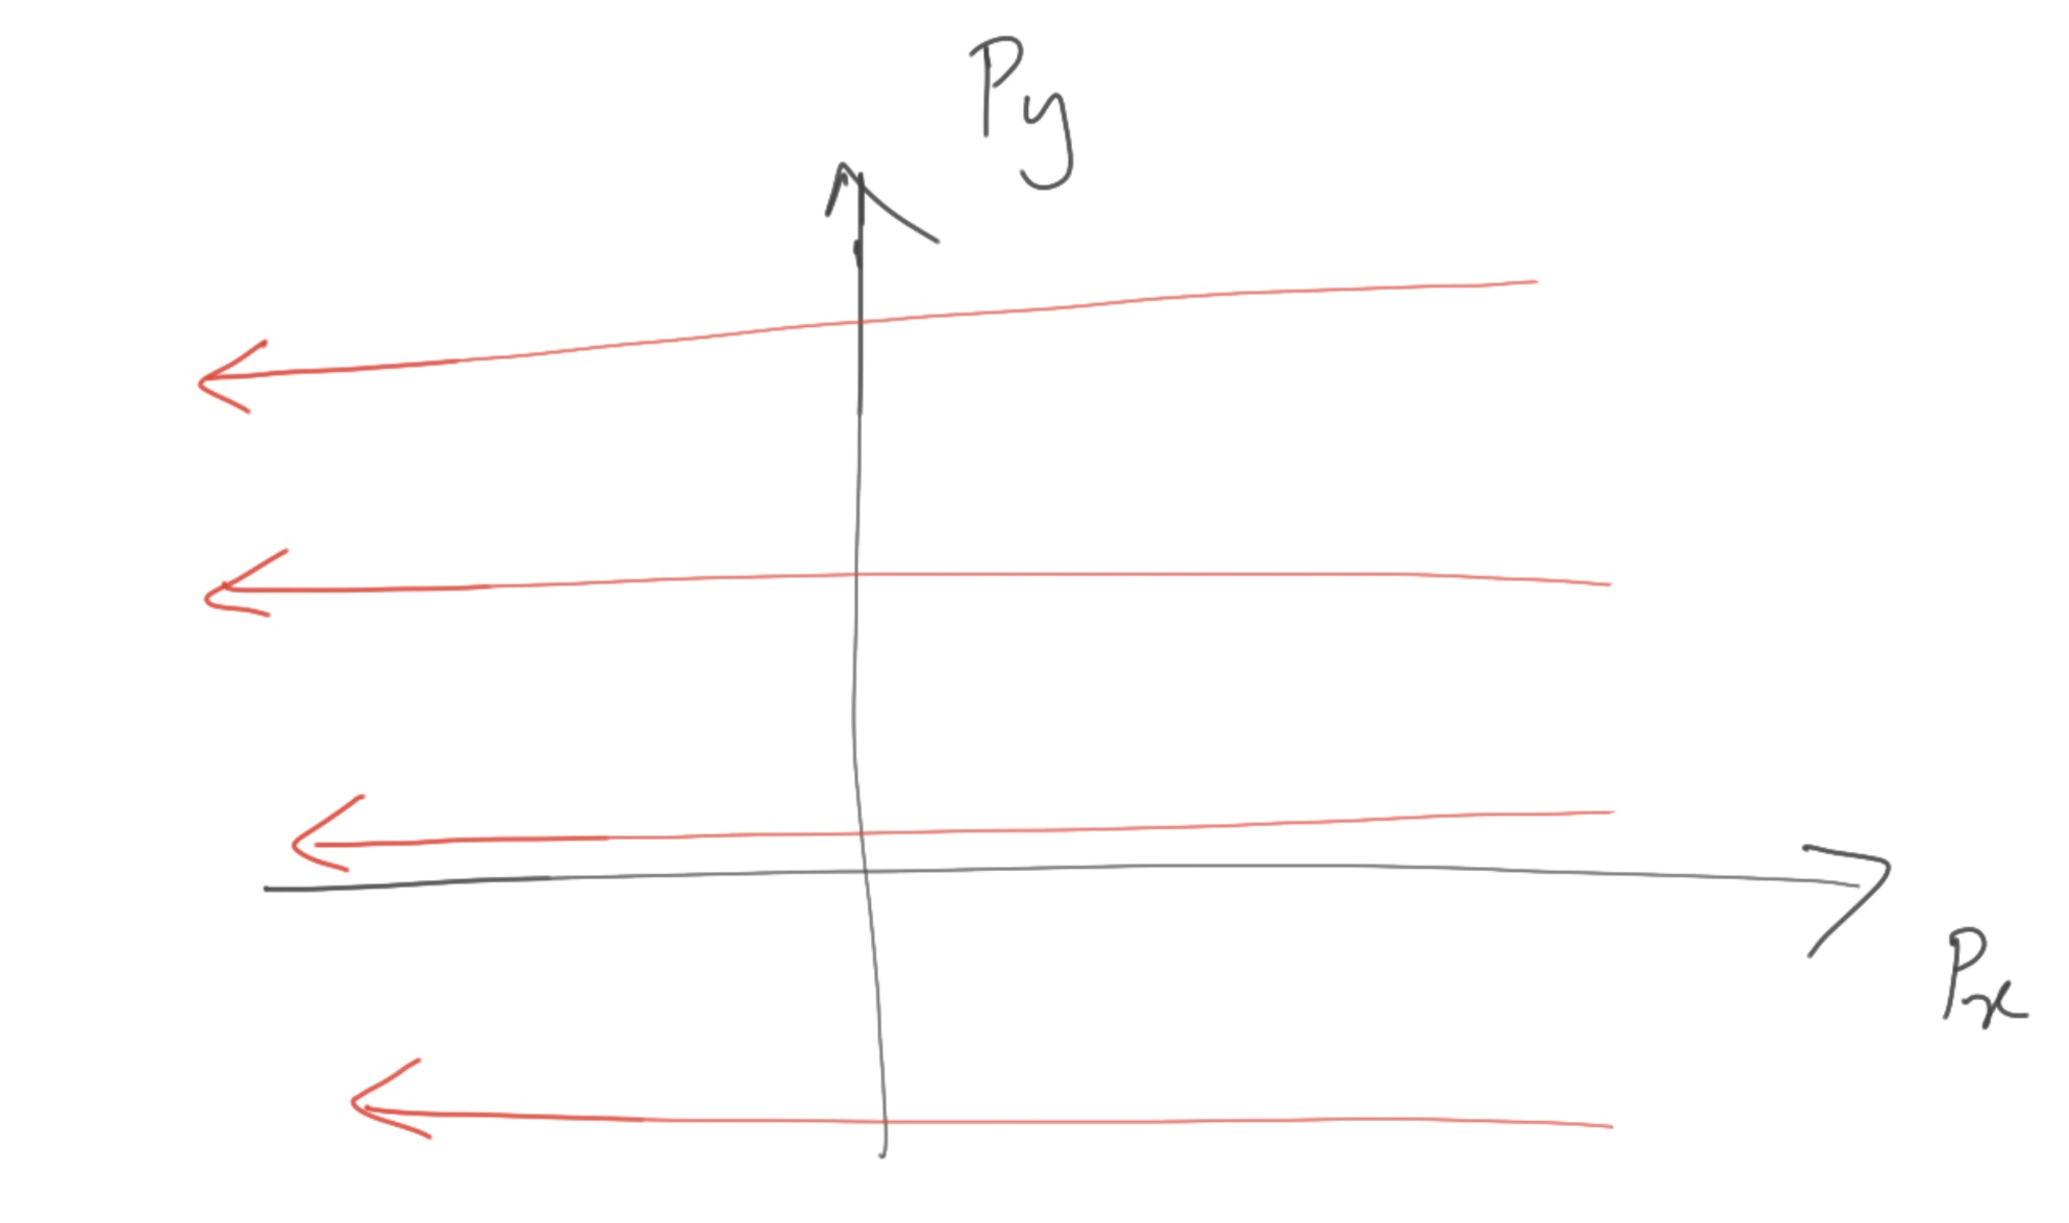
\includegraphics[width=0.4\linewidth]{Rx_flow}
  \caption{Pictorial representation of $R_x$ flow.
    \vspace{-1.em}
  }
  \label{Rx_flow}
\end{figure}



\begin{figure}
    \centering
  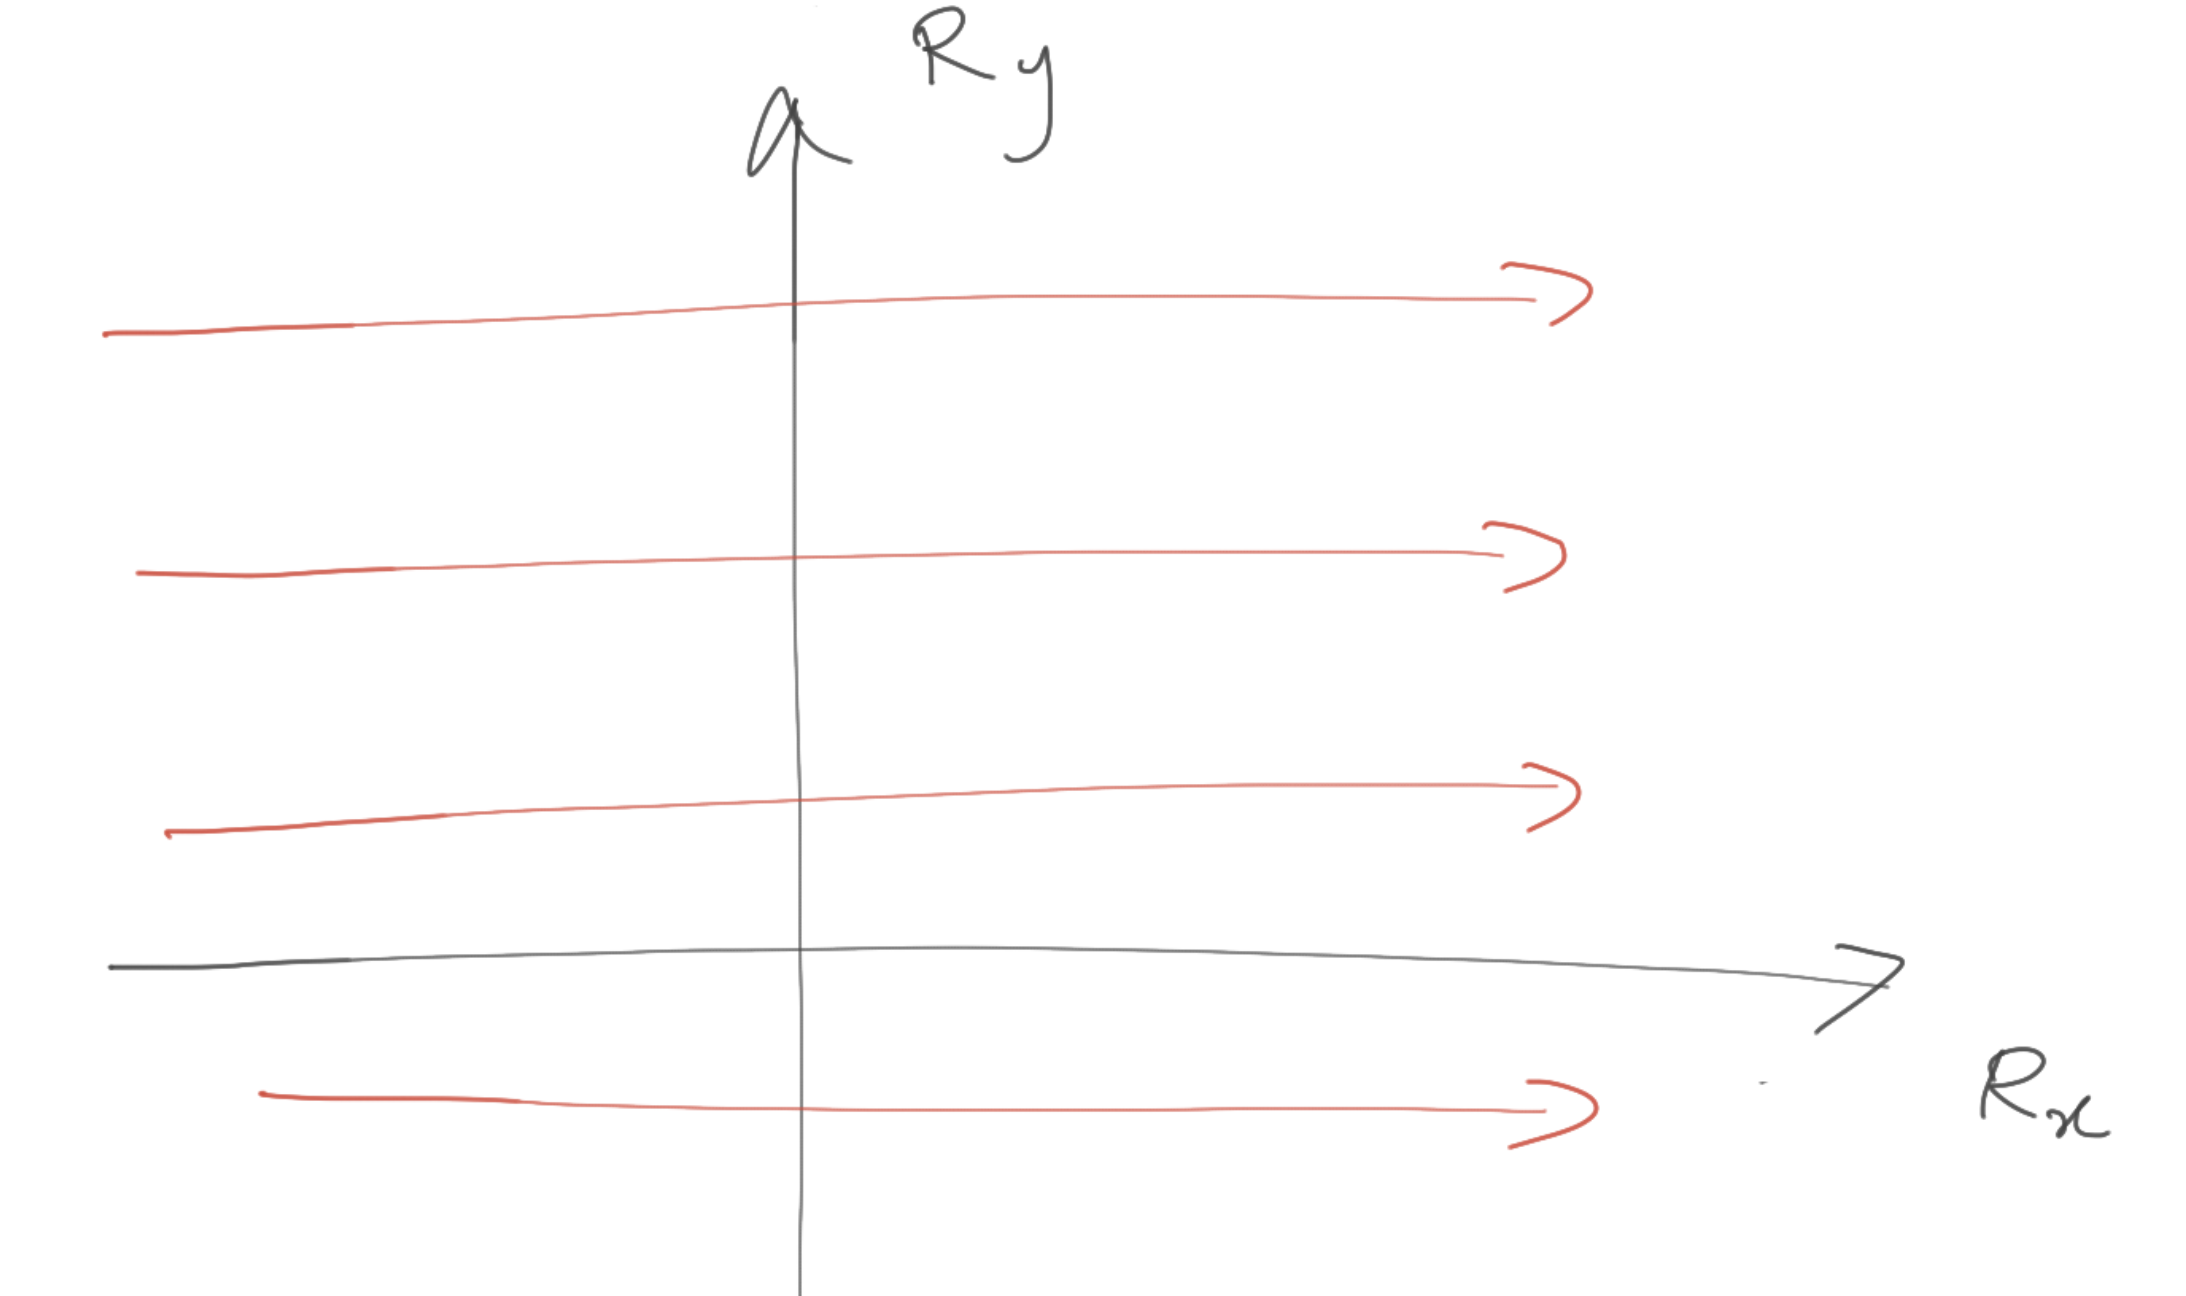
\includegraphics[width=0.4\linewidth]{Px_flow}
  \caption{Pictorial representation of $P_x$ flow.
    \vspace{-1.em}
  }
  \label{Px_flow}
\end{figure}



\begin{figure}
    \centering
  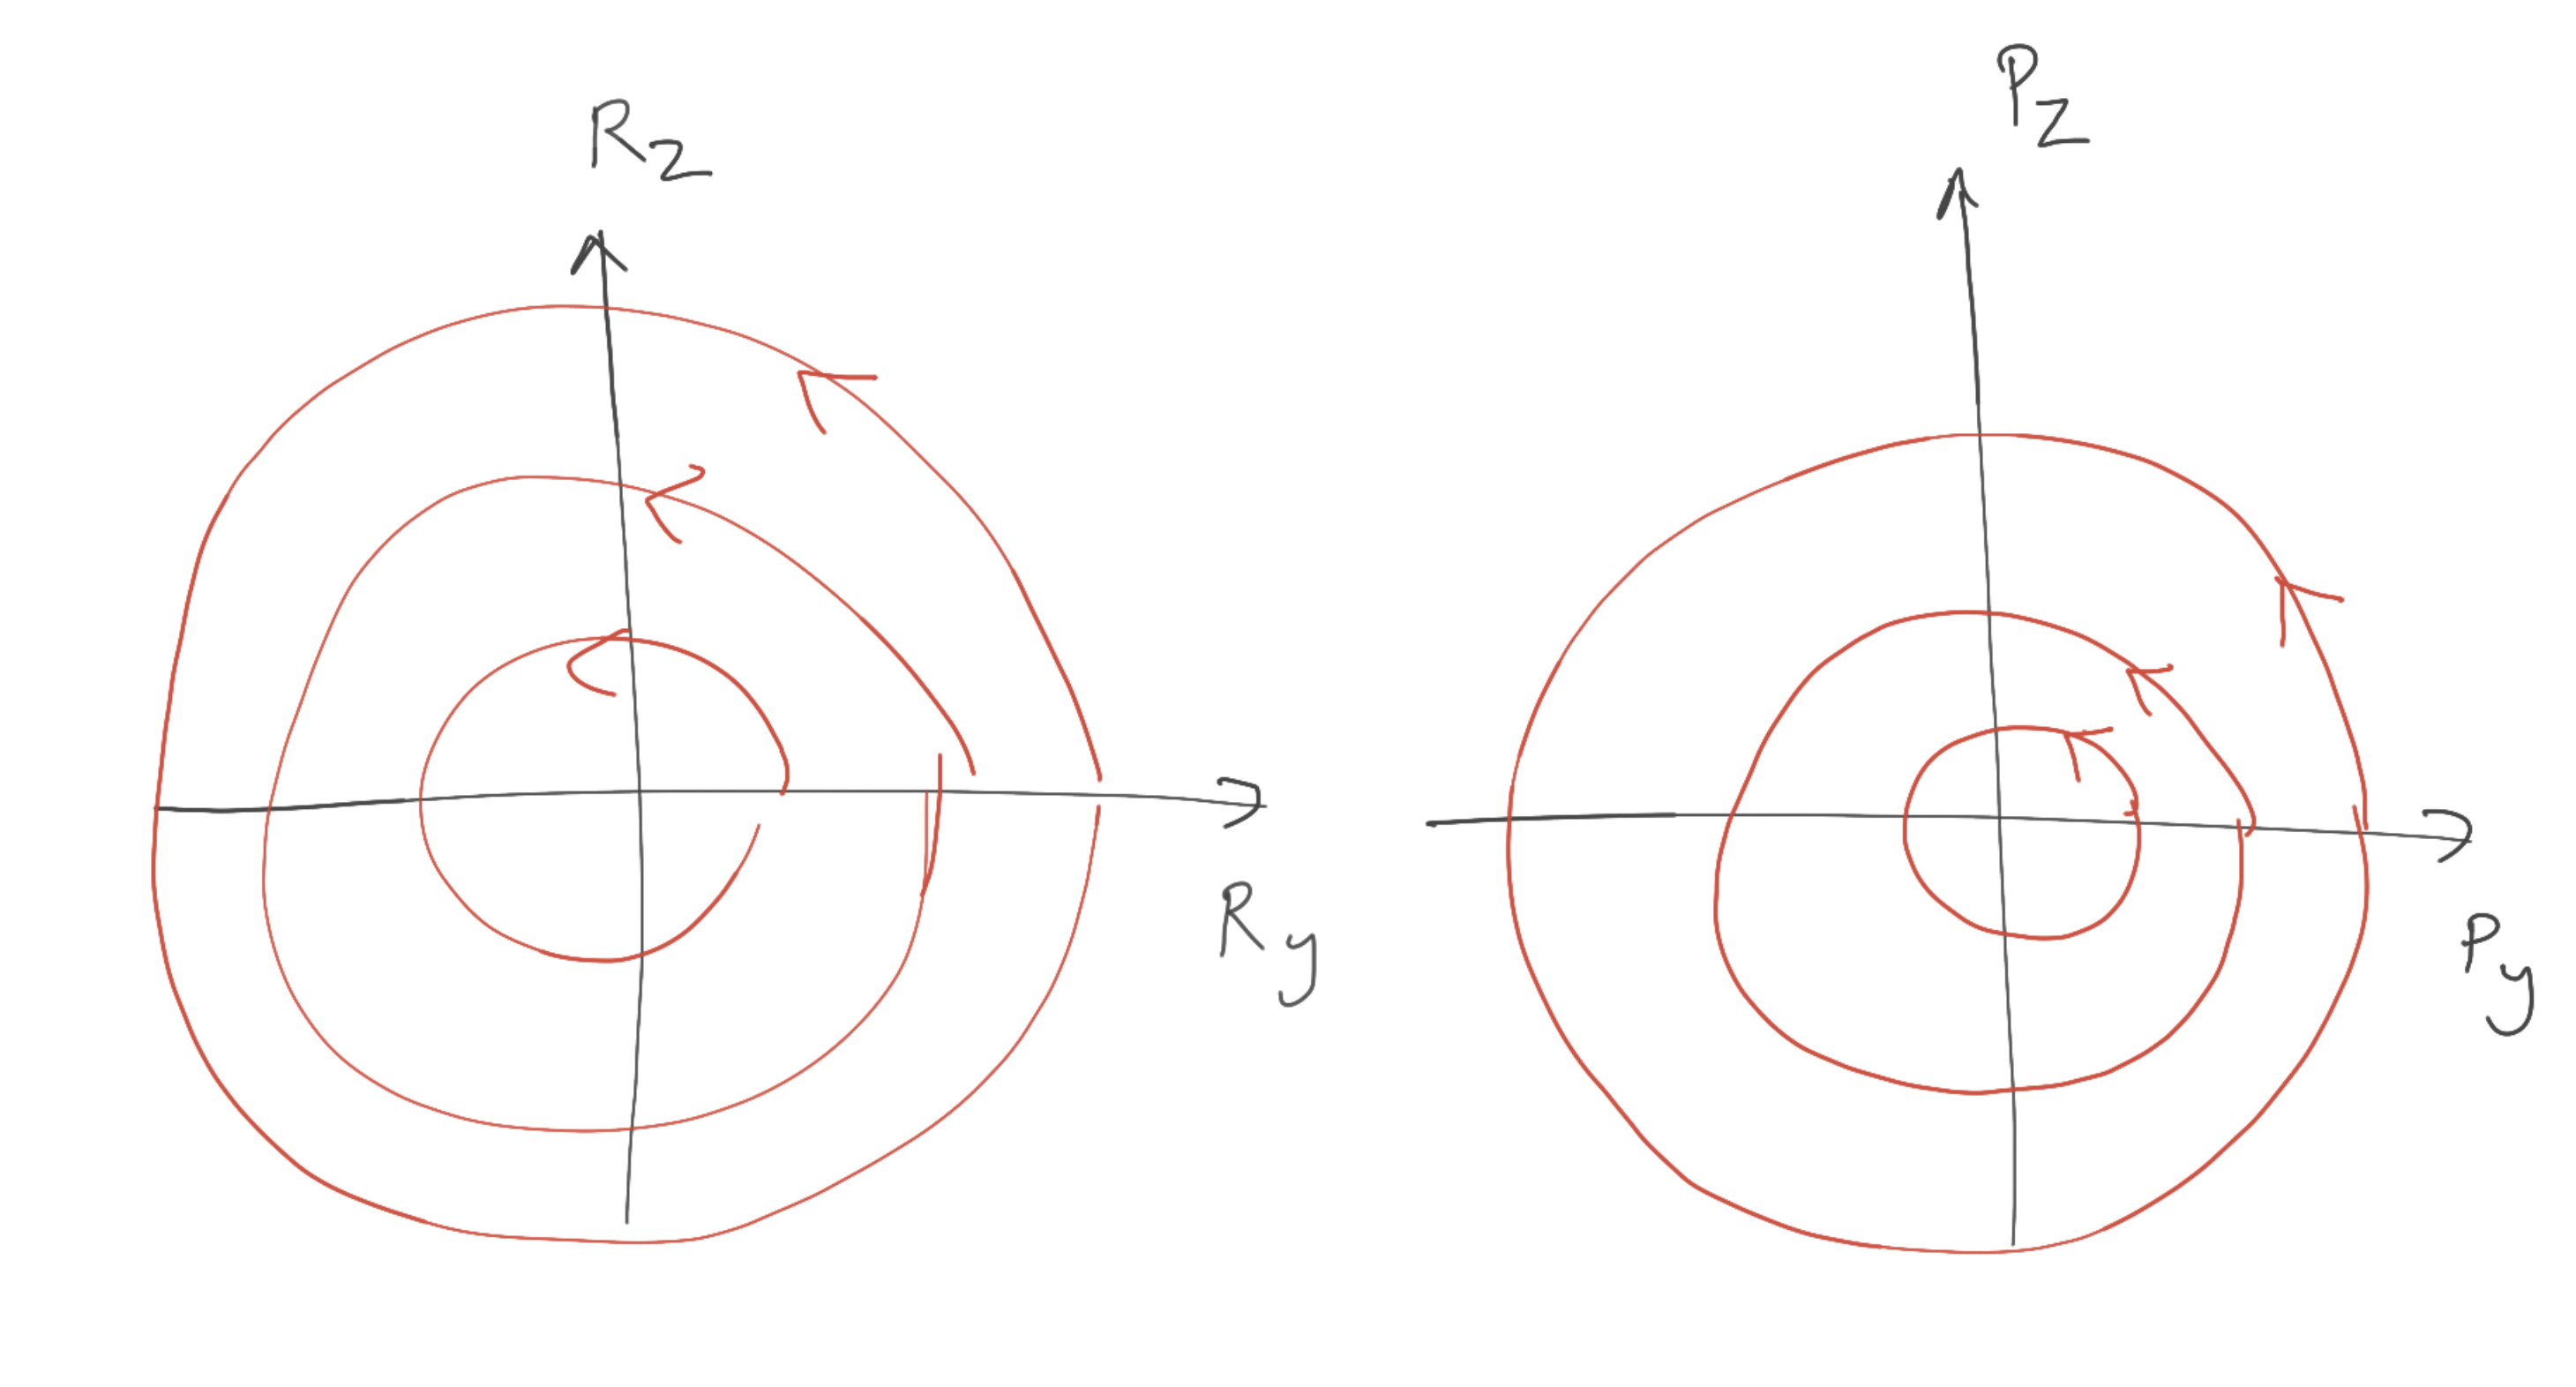
\includegraphics[width=0.4\linewidth]{Lx_flow}
  \caption{Pictorial representation of $L_x$ flow.
    \vspace{-1.em}
  }
  \label{Lx_flow}
\end{figure}



\begin{figure}
   \centering
  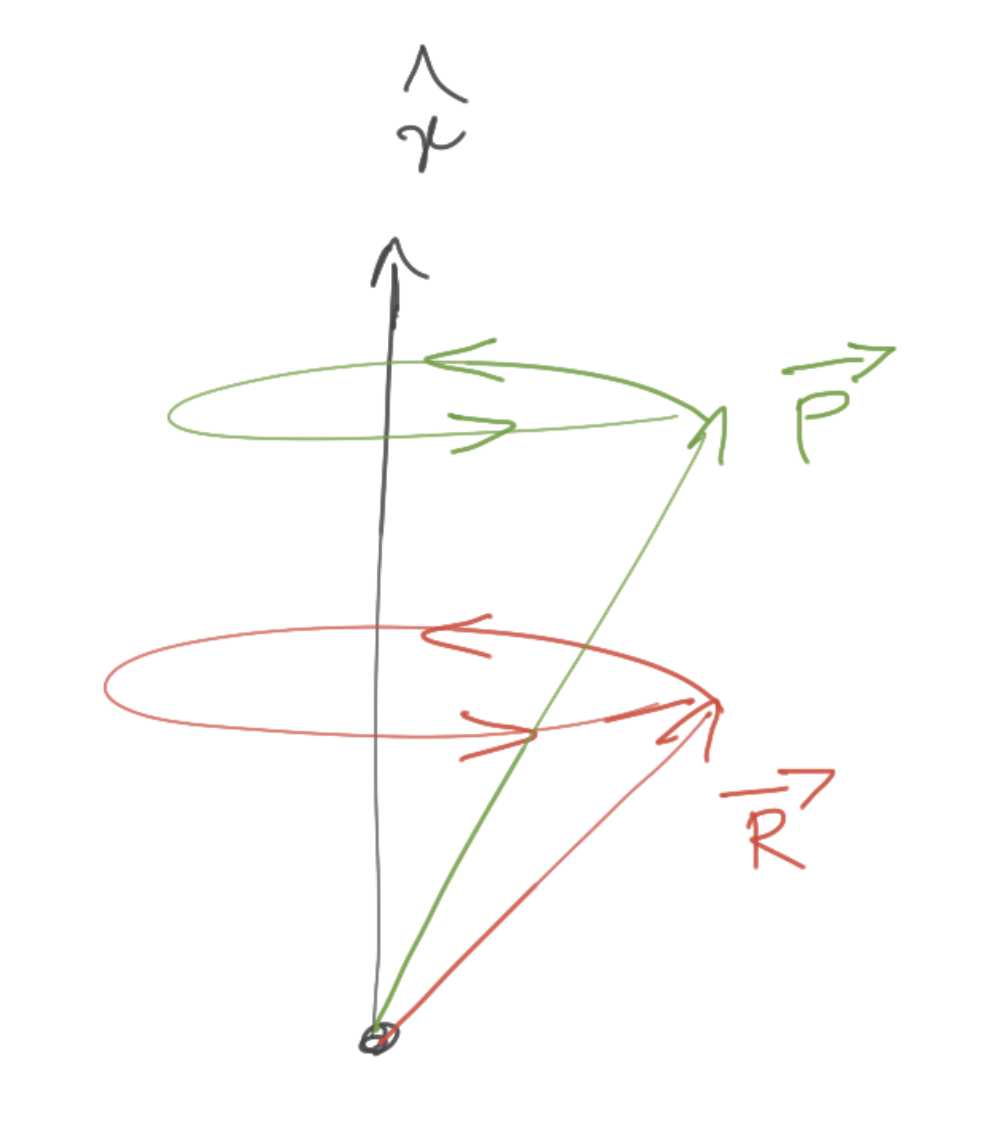
\includegraphics[width=0.4\linewidth]{Lx_flow_2}
  \caption{Pictorial representation of $L_x$ flow.
    \vspace{-1.em}
  }
  \label{Lx_flow_2}
\end{figure}




\begin{figure}
    \centering
  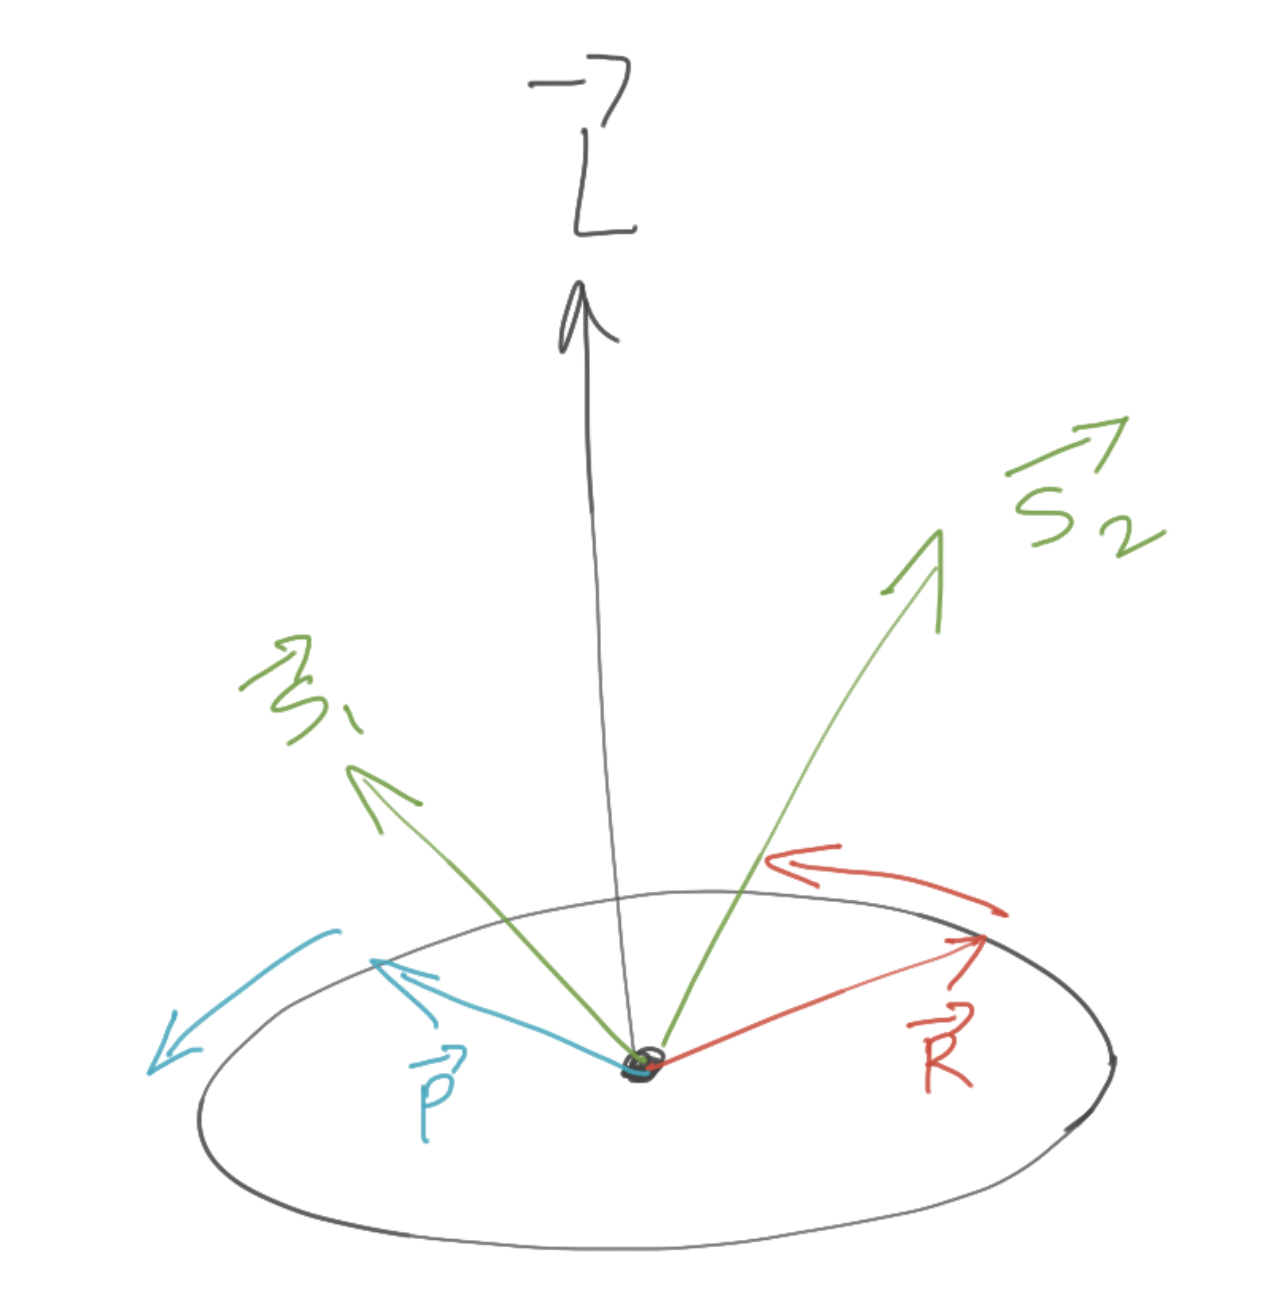
\includegraphics[width=0.4 \linewidth]{Lsq_flow}
  \caption{Pictorial representation of $L^2$ flow.
    \vspace{-1.em}
  }
  \label{Lsq_flow}
\end{figure}




\begin{figure}
  \centering
  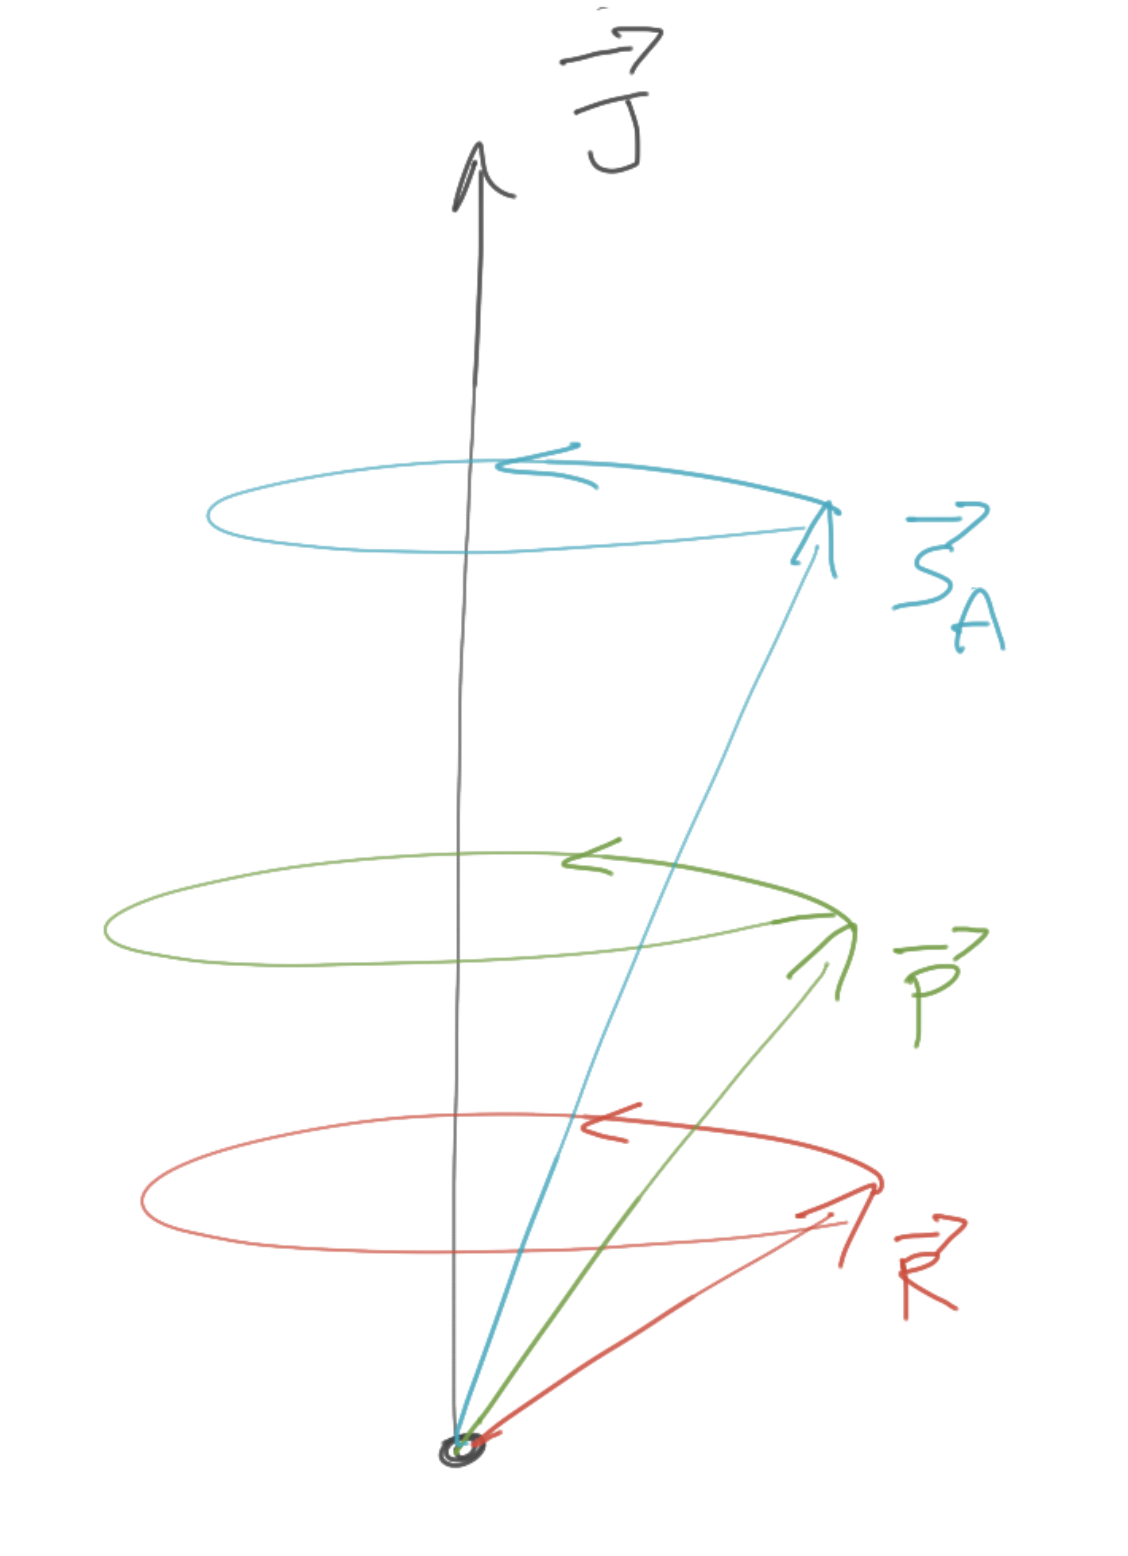
\includegraphics[width=0.4\linewidth]{Jsq_flow}
  \caption{Pictorial representation of $J^2$ flow.
    \vspace{-1.em}
  }
  \label{Jsq_flow}
\end{figure}




\section{Hamiltonian flow of the Hamiltonian}


Hamiltonian flow of the Hamiltonian is encoded in 
\begin{align}
\frac{d \vv{V}}{d \lambda}  =   \pb{\vv{V}, H},
\end{align}
which upon comparison with Eq.~\eqref{C0-EOM-PB} is found to
be the EOM of the system. The flow parameter $\lambda$ plays the role of
time $t$. In this sense, the Hamiltonian flow of the 
Hamiltonian is indeed special for the flow of the Hamiltonian
dictates the real time evolution of a system.
























